\section{はじめに}

% \begin{itemize}
%   \item わかるらんどの思想を述べる
%   \item 消去性コンピューティングについて\cite{kurihara2016}
% \end{itemize}

ワイヤレスネットワークや小型計算機の普及による
IoT社会が到来しつある現在、
人々は大量のリアルタイム情報や通知やメッセージなどに圧倒されている。
%
多くの情報を人間が理解しやすくするため、
以下のような視覚化手法が利用されている。

\vspace{3mm}

\begin{figure}[b]
\centering\fbox{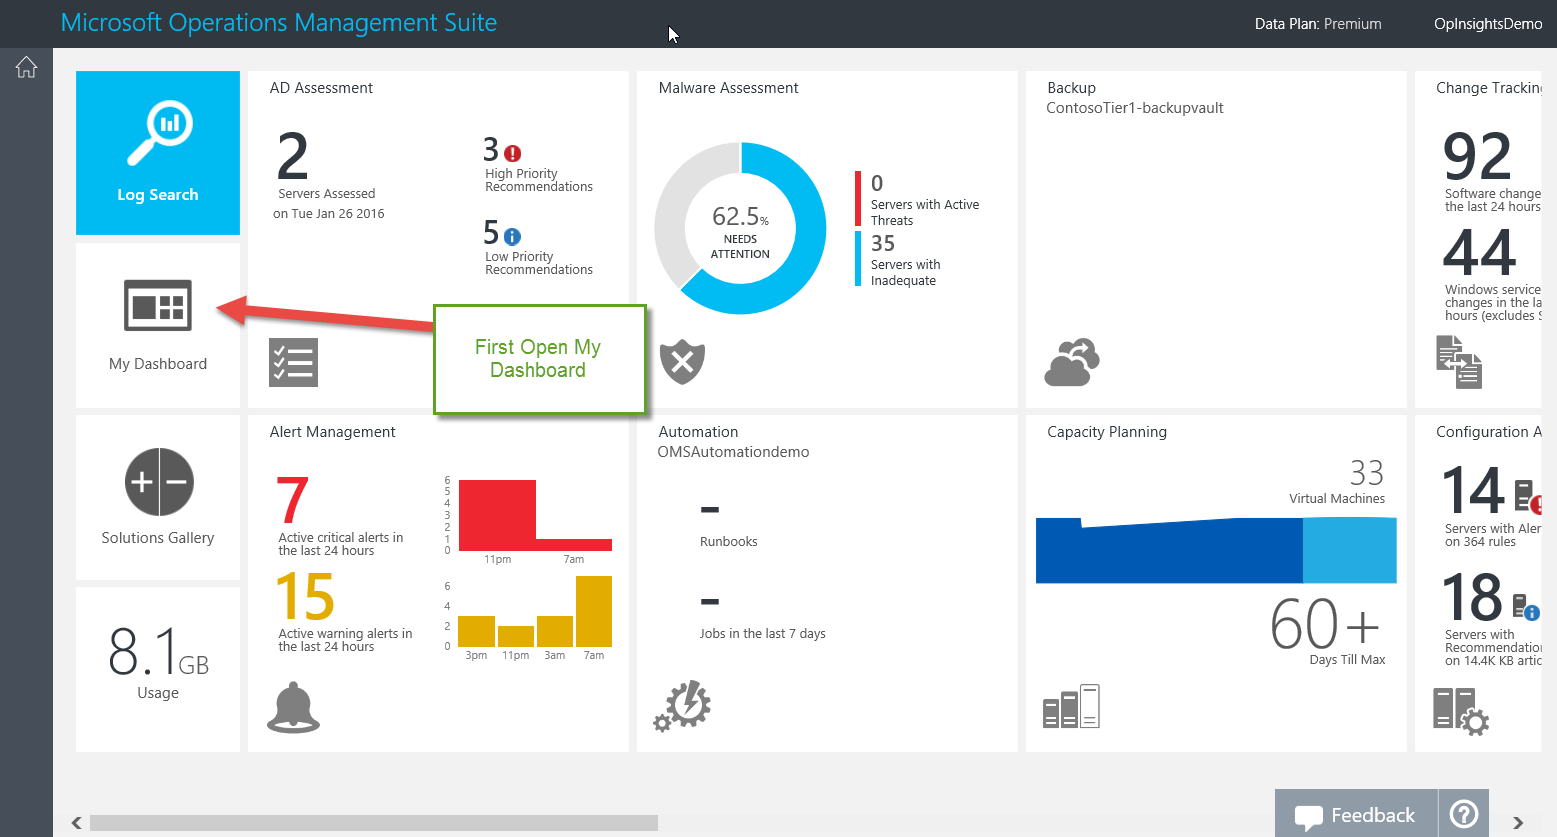
\includegraphics[width=7cm]{images/azure.png}}
\caption{Microsoft Azureの情報ダッシュボード}
\label{azure}
\end{figure}

\paragraph*{情報ダッシュボード}

情報ダッシュボード\cite{few}は、
複数のリアルタイム情報をタイル状に並べて表示することによって
多くの情報をわかりやすく視覚化するシステムである。
たとえばWindowsのスタート画面(図\ref{azure})の情報ダッシュボードには
天気予報や株価のようなリアルタイム情報を表示可能である。

% \vspace{2mm}
% \paragraph*{タイムライン表示}
% 
% Twitter, Facebook, LINEのような
% 近年のコミュニケーションシステムでは、
% 投稿を時系列に並べて表示する
% 「タイムライン表示」(図\ref{twitter})が広く利用されている。
% %
% タイムライン表示はリアルタイムに更新され、
% 時間順に情報を見るのには便利であるが、
% 投稿の多いユーザの記事ばかりが目立ちがちだし、
% 古い投稿がすぐに見えなくなってしまうという問題がある。
% 
% \begin{figure}[H]
% \centering\fbox{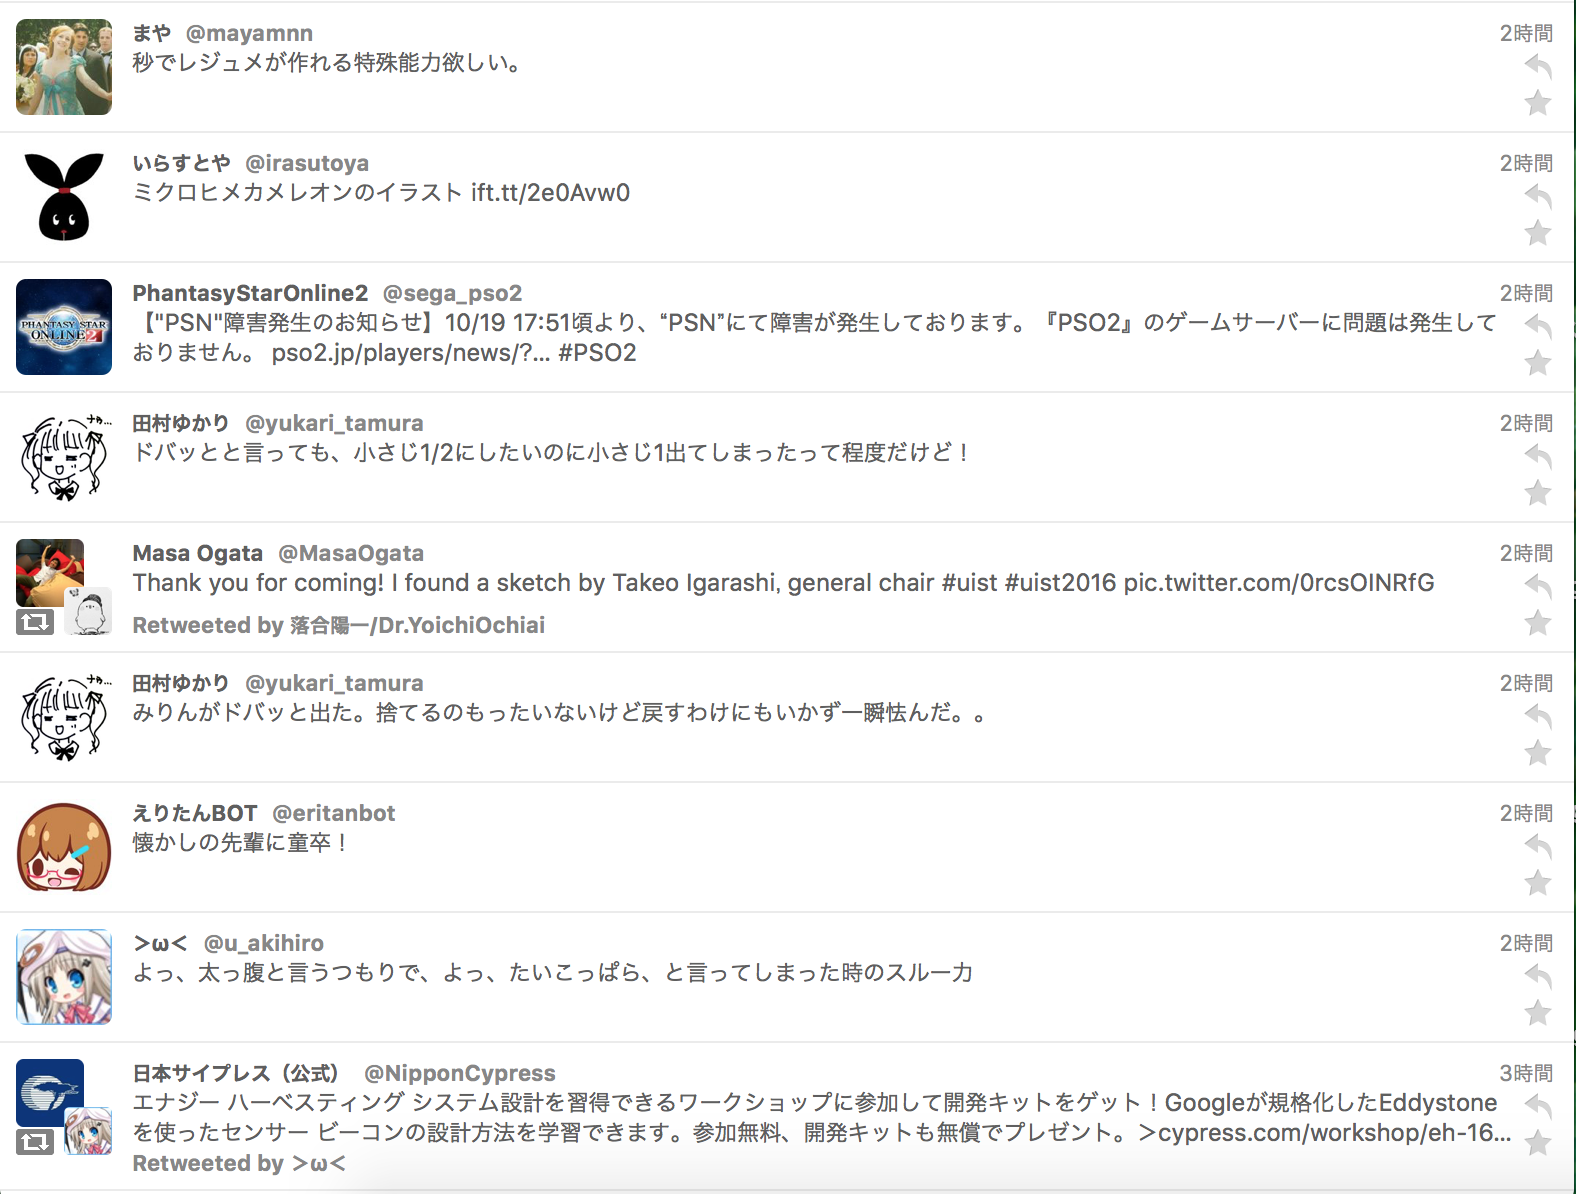
\includegraphics[width=7cm]{images/twitter.png}}
% \caption{Twitterのタイムライン}
% \label{twitter}
% \end{figure}

\vspace{2mm}
\paragraph*{スタンプ}

リアルタイムに流れていくタイムライン表示の中で情報を目立たせたいとき、
最近「スタンプ」と呼ばれるピクトグラムが
利用されることが多くなってきた(図\ref{linestamp})。

スタンプはテキストで記述するのが難しい表現や感情を伝えたり、
テキストを考えて入力するよりも速くて簡単であったりすることから、
近年LINEやFacebookメッセンジャー、オンラインゲームなどで広く利用されている。

\begin{figure}[H]
\centering\fbox{
\includegraphics[width=4cm]{images/linestamp.png}}
\caption{LINEのスタンプの例}
\label{linestamp}
\end{figure}

スタンプ的な表現を投稿可能な情報ダッシュボードを用意し、
その上で
ネット上の様々な情報や
ユーザの気分や感情を表示すれば、
現在の世界や人々の状況が一目了然になる。
%
実世界の状態や人間の状況を情報ダッシュボードにわかりやすく表示し、
かつ誰もが簡単に気分などをスタンプのように投稿して共有できる
「わかるらんど」システムを構築した。

% そこで、このスタンプをダッシュボードのセルに表示することで、
% ダッシュボードとスタンプベースのコミュニケーションを組み合わせた視覚化システム
% 『わかるらんど』を開発した。
% 『わかるらんど』は単純なアーキテクチャで、人の感情や現在の状況、
% IoT機器の情報などをリアルタイムに視覚化するシステムで、
% 非常に汎用なダッシュボードとして利用することができる。




